\documentclass[journal,12pt,twocolumn]{IEEEtran}

\usepackage{setspace}
\usepackage{gensymb}
\singlespacing
\usepackage[cmex10]{amsmath}

\usepackage{amsthm}

\usepackage{mathrsfs}
\usepackage{txfonts}
\usepackage{stfloats}
\usepackage{bm}
\usepackage{cite}
\usepackage{cases}
\usepackage{subfig}

\usepackage{longtable}
\usepackage{multirow}

\usepackage{enumitem}
\usepackage{mathtools}
\usepackage{steinmetz}
\usepackage{tikz}
\usepackage{circuitikz}
\usepackage{verbatim}
\usepackage{tfrupee}
\usepackage[breaklinks=true]{hyperref}
\usepackage{graphicx}
\usepackage{tkz-euclide}

\usetikzlibrary{calc,math}
\usepackage{listings}
    \usepackage{color}                                            %%
    \usepackage{array}                                            %%
    \usepackage{longtable}                                        %%
    \usepackage{calc}                                             %%
    \usepackage{multirow}                                         %%
    \usepackage{hhline}                                           %%
    \usepackage{ifthen}                                           %%
    \usepackage{lscape}     
\usepackage{multicol}
\usepackage{chngcntr}

\DeclareMathOperator*{\Res}{Res}

\renewcommand\thesection{\arabic{section}}
\renewcommand\thesubsection{\thesection.\arabic{subsection}}
\renewcommand\thesubsubsection{\thesubsection.\arabic{subsubsection}}

\renewcommand\thesectiondis{\arabic{section}}
\renewcommand\thesubsectiondis{\thesectiondis.\arabic{subsection}}
\renewcommand\thesubsubsectiondis{\thesubsectiondis.\arabic{subsubsection}}


\hyphenation{op-tical net-works semi-conduc-tor}
\def\inputGnumericTable{}                                 %%

\lstset{
%language=C,
frame=single, 
breaklines=true,
columns=fullflexible
}
\begin{document}

\newcommand{\BEQA}{\begin{eqnarray}}
\newcommand{\EEQA}{\end{eqnarray}}
\newcommand{\define}{\stackrel{\triangle}{=}}
\bibliographystyle{IEEEtran}
\raggedbottom
\setlength{\parindent}{0pt}
\providecommand{\mbf}{\mathbf}
\providecommand{\pr}[1]{\ensuremath{\Pr\left(#1\right)}}
\providecommand{\qfunc}[1]{\ensuremath{Q\left(#1\right)}}
\providecommand{\sbrak}[1]{\ensuremath{{}\left[#1\right]}}
\providecommand{\lsbrak}[1]{\ensuremath{{}\left[#1\right.}}
\providecommand{\rsbrak}[1]{\ensuremath{{}\left.#1\right]}}
\providecommand{\brak}[1]{\ensuremath{\left(#1\right)}}
\providecommand{\lbrak}[1]{\ensuremath{\left(#1\right.}}
\providecommand{\rbrak}[1]{\ensuremath{\left.#1\right)}}
\providecommand{\cbrak}[1]{\ensuremath{\left\{#1\right\}}}
\providecommand{\lcbrak}[1]{\ensuremath{\left\{#1\right.}}
\providecommand{\rcbrak}[1]{\ensuremath{\left.#1\right\}}}
\theoremstyle{remark}
\newtheorem{rem}{Remark}
\newcommand{\sgn}{\mathop{\mathrm{sgn}}}
\providecommand{\abs}[1]{\vert#1\vert}
\providecommand{\res}[1]{\Res\displaylimits_{#1}} 
\providecommand{\norm}[1]{\lVert#1\rVert}
%\providecommand{\norm}[1]{\lVert#1\rVert}
\providecommand{\mtx}[1]{\mathbf{#1}}
\providecommand{\mean}[1]{E[ #1 ]}
\providecommand{\fourier}{\overset{\mathcal{F}}{ \rightleftharpoons}}
%\providecommand{\hilbert}{\overset{\mathcal{H}}{ \rightleftharpoons}}
\providecommand{\system}{\overset{\mathcal{H}}{ \longleftrightarrow}}
	%\newcommand{\solution}[2]{\textbf{Solution:}{#1}}
\newcommand{\solution}{\noindent \textbf{Solution: }}
\newcommand{\cosec}{\,\text{cosec}\,}
\providecommand{\dec}[2]{\ensuremath{\overset{#1}{\underset{#2}{\gtrless}}}}
\newcommand{\myvec}[1]{\ensuremath{\begin{pmatrix}#1\end{pmatrix}}}
\newcommand{\mydet}[1]{\ensuremath{\begin{vmatrix}#1\end{vmatrix}}}
\numberwithin{equation}{subsection}
\makeatletter
\@addtoreset{figure}{problem}
\makeatother
\let\StandardTheFigure\thefigure
\let\vec\mathbf
\renewcommand{\thefigure}{\theproblem}
\def\putbox#1#2#3{\makebox[0in][l]{\makebox[#1][l]{}\raisebox{\baselineskip}[0in][0in]{\raisebox{#2}[0in][0in]{#3}}}}
     \def\rightbox#1{\makebox[0in][r]{#1}}
     \def\centbox#1{\makebox[0in]{#1}}
     \def\topbox#1{\raisebox{-\baselineskip}[0in][0in]{#1}}
     \def\midbox#1{\raisebox{-0.5\baselineskip}[0in][0in]{#1}}
\vspace{3cm}
\title{Assignment 1}
\author{Omkaradithya R Pujari - AI20BTECH11017}
\maketitle
\newpage
\bigskip
\renewcommand{\thefigure}{\theenumi}
\renewcommand{\thetable}{\theenumi}
Download all python codes from 
\begin{lstlisting}
https://github.com/Omkaradithya/EE3900-Linear-Systems-and-Signal-Processing/blob/main/Assignment%201/ramsey%201.1.5.py
\end{lstlisting}
%
and latex codes from 
%
\begin{lstlisting}
https://github.com/Omkaradithya/EE3900-Linear-Systems-and-Signal-Processing/blob/main/Assignment%201/assgn1.tex
\end{lstlisting}
\section*{\textbf{Problem}}
\textbf{(Ramsey - 1.1.5)} Plot the points \myvec{0 \\ 2}, \myvec{1 \\ 1}, \myvec{4 \\ 4} and \myvec{3\\5} and prove that they are vertices of a rectangle.
\section*{\textbf{Solution}}
Let,
\begin{align}
    \vec{A} = \myvec{0 \\ 2},
\end{align}
\begin{align}
    \vec{B} = \myvec{1 \\ 1}, 
\end{align}
\begin{align}    
    \vec{C} = \myvec{4 \\ 4}
\end{align}
\begin{align}
    \vec{D} = \myvec{3 \\ 5}
\end{align}

The direction vector are calculated as follows:
\begin{align}
\vec{B-A} = \myvec{1-0 \\ 1-2}
= \myvec{1 \\ -1}
\end{align}
\begin{align}
\vec{C-B} = \myvec{4-1 \\ 4-1}
= \myvec{3 \\ 3}
\end{align}
\begin{align}
\vec{D-C} = \myvec{3-4 \\ 5-4}
= \myvec{-1 \\ 1}
\end{align}
\begin{align}
\vec{A-D} = \myvec{0-3 \\ 2-5}
= \myvec{-3 \\ -3}
\end{align}

Since the directional vectors AB (B-A) and CD (D-C) are in the same ratio, AB and CD are parallel and opposite to each other. Similarly, directional vectors BC (C-B) and DA (A-D) are also parallel and opposite to each other. Since the opposites sides are parallel, the given points are vertices of a parallelogram.
Also, 
\begin{align}
\vec{(B - A)}^T \vec{(C - D)} = \myvec{1  -1} \myvec{ 1 \\ -1}
\end{align}
\begin{align}
= 0
\end{align}
 Therefore $$\angle ABC = 90^o$$ and hence, the points A,B,C and D are vertices of a rectangle.
 
\begin{figure}[!ht]
\centering
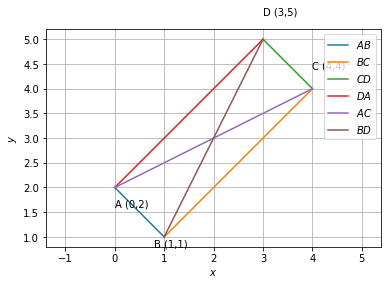
\includegraphics[width=\columnwidth]{plot.png}
\caption{Plot of the points}
\label{Plot}
\end{figure}
\end{document}
